\documentclass[12pt]{article}
\usepackage[czech]{babel}
\usepackage[utf8]{inputenc}
\usepackage[plainpages=false,pdfpagelabels,unicode]{hyperref}
\usepackage[pdftex]{graphicx}
\usepackage[margin=2cm, includefoot]{geometry}

\begin{document}

\title{Experimentální metody a~speciální praktikum \\
Měření optických vlastností tenkých vrstev}

\author{Vlasta Štěpánová a~Pavel Ondračka}
\maketitle

\section{Úvod}
Optické metody charakterizace tenkých vrstev poskytují celou řadu informací o~vlastnostech vrstev. V oblasti ultrafialového (UV) až viditelného záření jsou důležité pro mnohé aplikace jejich optické konstanty (index lomu a~extinkční koeficient). Je rovněž možné zjistit jejich tloušťku a~parametry elektronové struktury. V infračervené oblasti poskytuje absorpce ve vrstvách informace o~chemických vazbách, tudíž i o~složení a~struktuře vrstev.

\section{Teorie}

Na rozhraní dvou prostředí s rozdílnými indexy lomu se světlo láme dle Snellova zákona
\begin{equation}
\hat{n}_0 \sin\hat{\theta}_0 = \hat{n}_1 \sin\hat{\theta}_1 \mathrm{.}
\end{equation}
Fresnelovy koeficienty na~rozhraní jsou pro s polarizovanou vlnu: 
\begin{equation}
\hat{r}_\mathrm{s} = \frac{ \hat{n}_0 \cos \hat{\theta}_0 - \hat{n}_1 \cos \hat{\theta}_1}{ \hat{n}_0 \cos \hat{\theta}_0 + \hat{n}_1 \cos \hat{\theta}_1}  \mathrm{,}
\end{equation}
pro p polarizovanou vlnu: 
\begin{equation}
\hat{r}_\mathrm{p} = \frac{ \hat{n}_0 \cos \hat{\theta}_1 - \hat{n}_1 \cos \hat{\theta}_0}{ \hat{n}_0 \cos \hat{\theta}_1 + \hat{n}_1 \cos \hat{\theta}_0}  \mathrm{.}
\end{equation}
Indexy lomu jsou obecně komplexní ($\hat{n}_i = n_i + \mathrm{i} \kappa_i$).

\begin{figure}
  \centering
  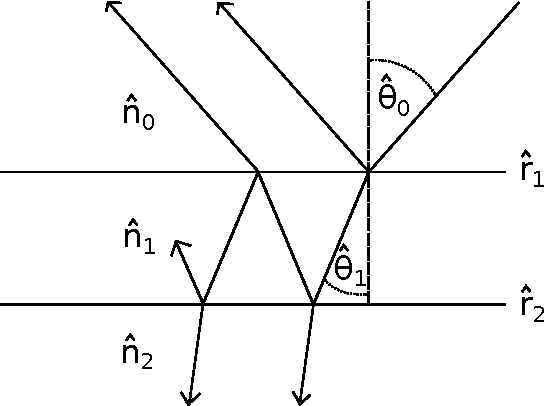
\includegraphics[width=80mm]{schema.pdf}
  \caption{Schéma rozhraní vzduch--vrstva--substrát}
  \label{schema}
\end{figure}


\subsection{Elipsometrie}
Princip elipsometrie spočívá ve studiu změn polarizačního stavu světla po odrazu od zkoumaného vzorku. Tato změna se obvykle vyjadřuje jako tzv. elipsometrický poměr $\hat{\rho}$, který je definován jako:
\begin{equation} \hat{\rho} = \frac{\hat{r}_\mathrm{p}}{\hat{r}_\mathrm{s}} \;\;\; \mathrm{nebo} \;\;\; \hat{\rho} = \frac{\hat{t}_\mathrm{p}}{\hat{t}_\mathrm{s}} \mathrm{,}\label{elpomer}\end{equation}
kde $\hat{r}_\mathrm{s}$ a~$\hat{r}_\mathrm{p}$ jsou Frenelovy koeficienty odrazu a~$\hat{t}_\mathrm{s}$ a~$\hat{t}_\mathrm{p}$ jsou Frenelovy koeficienty průchodu pro s a~p polarizovanou vlnu. Elipsometrický poměr můžeme vyjádřit pomocí elipsometrických parametrů $\Psi$ (azimut) a~$\Delta$ (fázový posun) jako:
%
\begin{equation} \hat{\rho} = \tan{\Psi} \; \mathrm{e}^{\mathrm{i}\Delta} \mathrm{.}\end{equation}
%
V přiblížení dvoufázového systému (okolí--polonekonečný vzorek) můžeme komplexní index lomu určit přímo z elipsometrického poměru jako
\begin{equation} \hat{n}_1 = \hat{n}_0 \sin \hat{\theta}_0 \sqrt{1 + \tan^2 \hat{\theta}_0 \left(\frac{1 - \hat{\rho}}{1 + \hat{\rho}} \right)^2  } \, \mathrm{.} \label{ellrov} \end{equation}

%
Při fázově modulované elipsometrii používáme elipsometr v~konfigurace polarizátor -- kompenzátor -- substrát -- analyzátor nebo polarizátor -- substrát -- kompenzátor -- analyzátor, přičemž polarizátor, kompenzátor a~analyzátor jsou vůči sobě v~zafixovaných pozicích. Fázové zpoždění kompenzátoru $\delta$ je periodickou funkcí času. Pokud azimutální úhly použitých komponent splňují vztahy $P - C = \pm \pi/4$, $C=0, \pi/2$ a~$A = \pm \pi/4$, pak pro světelný tok $I$ na~detektoru můžeme psát:
%
\begin{equation} I(t) \propto 1 + I_\mathrm{s} \sin{\delta(t)} + I_\mathrm{c} \cos{\delta(t)} \mathrm{.}\end{equation}
%
Fourierovskou analýzou periodického signálu $I(t)$ jsou získány přidružené elipsometrické parametry $I_\mathrm{s}$ a~$I_{\mathrm{c}}$, pro které platí:
\begin{equation} I_\mathrm{s} = \sin{2\Psi} \sin{\Delta} \mathrm{.}\end{equation}
$I_{\mathrm{c}}$ záleží na~konfiguraci komponent, pokud je $P - C = A = \pi/4$ a~$ C = 0 $, jedná se o~takzvanou konfiguraci II:
\begin{equation} I_\mathrm{cII} = \sin{2\Psi} \cos{\Delta} \mathrm{,}\end{equation} 
při $P - C = A = C = \pi/4$ se jedná o~takzvanou konfiguraci III:
\begin{equation} I_\mathrm{cIII} = \cos{2\Psi} \mathrm{.}\end{equation}

\subsubsection{Jobin-Yvon UVISEL}
Elipsometr Jobin-Yvon UVISEL je schématicky znázorněn na~schématu \ref{fig:elipsometrimg}.  Měřící rozsah tohoto přístroje je od 190\,nm do 2000\,nm. Hlavy elipsometru jsou umístěny na~goniometru, měření může být tudíž prováděno pod různými úhly. Běžně se měří úhly dopadu 55$^\circ$, 60$^\circ$, 65$^\circ$, 70$^\circ$ a~75$^\circ$. Jedná se o~fázově modulovaný elipsometr. Měření probíhá tak, že z lampy L vychází  nepolarizované světlo, které poté jde přes polarizátor P, kde dojde k jeho lineární polarizaci, odráží se od vzorku a~přes kompenzátor C, analyzátor A a~monochromátor dopadá na~detektor D.


\begin{figure}
  \centering
  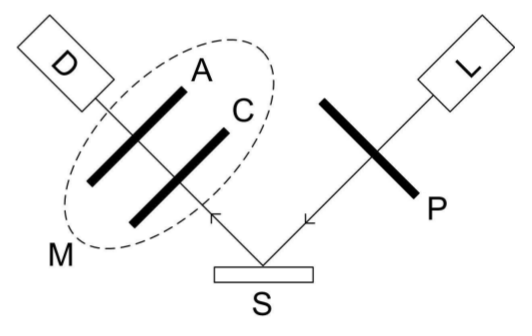
\includegraphics[width=120mm]{schema-elipsometru.png}
  \caption{Schéma elipsometru UVISEL (P--polarizátor, C--kompenzátor, D--detektor, L--lampa, M--modulátor, A--analyzátor, S--substrát).}
  \label{fig:elipsometrimg}
\end{figure}


\subsection{Viditelná a~UV spektroskopická reflektometrie}
Odrazivost R je definována jako průměr odrazivostí pro s a~p polarizované světlo 
%
\begin{equation} R = \frac{1}{2}(R_\mathrm{s} + R_\mathrm{p})\, \mathrm{,}\end{equation}
%
kde $R_\mathrm{s} = |\hat{r}_\mathrm{s}|^2$, $R_\mathrm{p} = |\hat{r}_\mathrm{p}|^2$.
Pro celkovou odrazivost systému vzduch--vrstva--substrát (obrázek \ref{schema}) platí 
\begin{equation} R = \left|\frac{\hat{r}_1 + \hat{r}_2 \mathrm{e}^{\mathrm{i}\hat{\alpha}} }{1 + \hat{r}_1 \hat{r}_2 \mathrm{e}^{\mathrm{i}\hat{\alpha}}}\right|^2 \mathrm{,} \label{Rvzo}\end{equation}
%
kde $\hat{\alpha}$ je fázový rozdíl paprsku  
\begin{equation} \hat{\alpha} = \frac{ 4 \pi d \hat{n}_1}{\lambda} \mathrm{,}\end{equation}
%
$d$ je tloušťka vrstvy a~$\lambda$ je vlnová délka světla. 

Při spektroskopické reflektometrii měříme spektrální závislost poměru intenzity dopadajícího $I_\mathrm{i}$ a~odraženého světla $I_\mathrm{r}$.
%
\begin{equation} R = \frac{I_\mathrm{r}}{I_\mathrm{i}} = \frac{|\hat{E}_\mathrm{r}|^2}{|\hat{E}_\mathrm{i}|^2}\end{equation}
%
Spektrofotometr může být buď jednokanálový, nebo dvoukanálový. V tomto praktiku byl používán dvoukanálový spektrofotometr. V použitém dvoukanálovém spektrofotometru je jeden zdroj záření, ale poté je paprsek rozdělen na~dva kanály a~každý kanál má vlastní detektor. První kanál je vzorkový, druhý referenční. Pro měřené intenzity na~vzorkovém kanále $I_\mathrm{s1}$ a~referenčním kanále $I_\mathrm{r1}$ můžeme psát:
%
\begin{equation} I_\mathrm{s1} = R_\mathrm{n} Z_1 D_\mathrm{s1} G_\mathrm{n} \mathrm{,}\;\;\;\;\;\; I_{r1} = R_\mathrm{r} Z_1 D_\mathrm{r1} G_\mathrm{r} \mathrm{,}\end{equation}
%
kde $R_\mathrm{n}$ a~$R_\mathrm{r}$ jsou odrazivosti vzorků, $Z_1$ je aktuální intenzita zdroje v~čase měření, $D_\mathrm{s1}$ a~$D_\mathrm{r1}$ citlivost detektoru v~čase měření a~$G_\mathrm{s}$,$G_\mathrm{r}$ jsou geometrické faktory pro jednotlivé kanály, které zahrnují například různé polohy (naklonění) vzorků a~různé technické provedení obou kanálů (například polopropustné zrcadlo nemusí propouštět na~oba dva kanály stejně světla). 

Je vidět, že již z těchto dvou měření, za předpokladu znalosti odrazivosti jednoho ze~vzorků, by šla určit odrazivost druhého. Problém je, že ve výsledku by vystupoval poměr $G_\mathrm{s}/G_\mathrm{r}$ a~geometrické faktory, které se na~obou kanálech mohou značně lišit, nejdou určit. Proto se provádí měření dvě. Poprvé je na~vzorkový kanál umístěn vzorek normálový se známou odrazivostí. Na~referenční kanál je umístěn vzorek referenční, můžeme použít libovolné zrcadlo. Při druhém měření umístíme na~vzorkový kanál vzorek, který chceme změřit, a~druhý kanál ponecháme beze změny. Pro naměřené intenzity při druhém měření platí:
\begin{equation} I_{s2} = R Z_2 D_\mathrm{s2} G_\mathrm{s} \;\;\;\;\;\; I_{r2} = R_\mathrm{r} Z_2 D_\mathrm{r2} G_\mathrm{r} \mathrm{,}\end{equation}
kde $R$ je odrazivost vzorku, který chceme změřit, $G_\mathrm{s}$ je geometrický faktor měřeného vzorku, index 2 u ostatních veličin značí druhé měření. Zkombinováním všech rovnic získáme:
\begin{equation}  \displaystyle\frac{\displaystyle\frac{I_{s2}}{I_{r2}} }{\displaystyle\frac{I_{s1}}{I_{r1}} } = \frac{R}{R_\mathrm{n}} \frac{G_\mathrm{s}}{G_n}\frac{D_\mathrm{s2}}{D_\mathrm{s1}}\frac{D_\mathrm{r2}}{D_\mathrm{r1}}\mathrm{.}\end{equation}

Ve výsledném vztahu nevystupují fluktuace zdroje a~geometrický faktor na~druhém kanálu, protože byl pro obě měření stejný. Poměr $G_\mathrm{s}/G_n$ je blízký jedné, protože se jedná o~stejný kanál, pouze vzorky jsou různé. Proměnlivé citlivosti detektorů se dají vykompenzovat vyšším počtem měření. Pokud $G_\mathrm{s} = G_n$ a~citlivost detektorů se v~čase nemění, získáme jednoduchý vzorec:
\begin{equation}R = R_\mathrm{n} \frac{\displaystyle\frac{I_{s2}}{I_{r2}} }{\displaystyle\frac{I_{s1}}{I_{r1}} } \mathrm{.}\end{equation}

\subsubsection{LAMBDA 45 UV/VIS}
LAMBDA 45 je spektrofotometr od firmy PerkinElmer vybavený monochromátorem s měřícím rozsahem v~rozmezí 190--1100\,nm. Zdrojem světla pro viditelnou a~blízkou UV oblast je halogenová lampa, pro UV oblast lampa deuteriová. Udávaná přesnost vlnové délky je $\pm$ 0,1\,nm. Jedná se o~dvoukanálový spektrofotometr, tj. svazek světla je rozdělen na~dva kanály, jeden jde na~referenční vzorek (zrcadlo), kde se zjišťuje aktuální intenzita paprsku, a~druhá část dopadá na~vzorek. Každý kanál má svůj detektor.

\begin{figure}
  \centering
  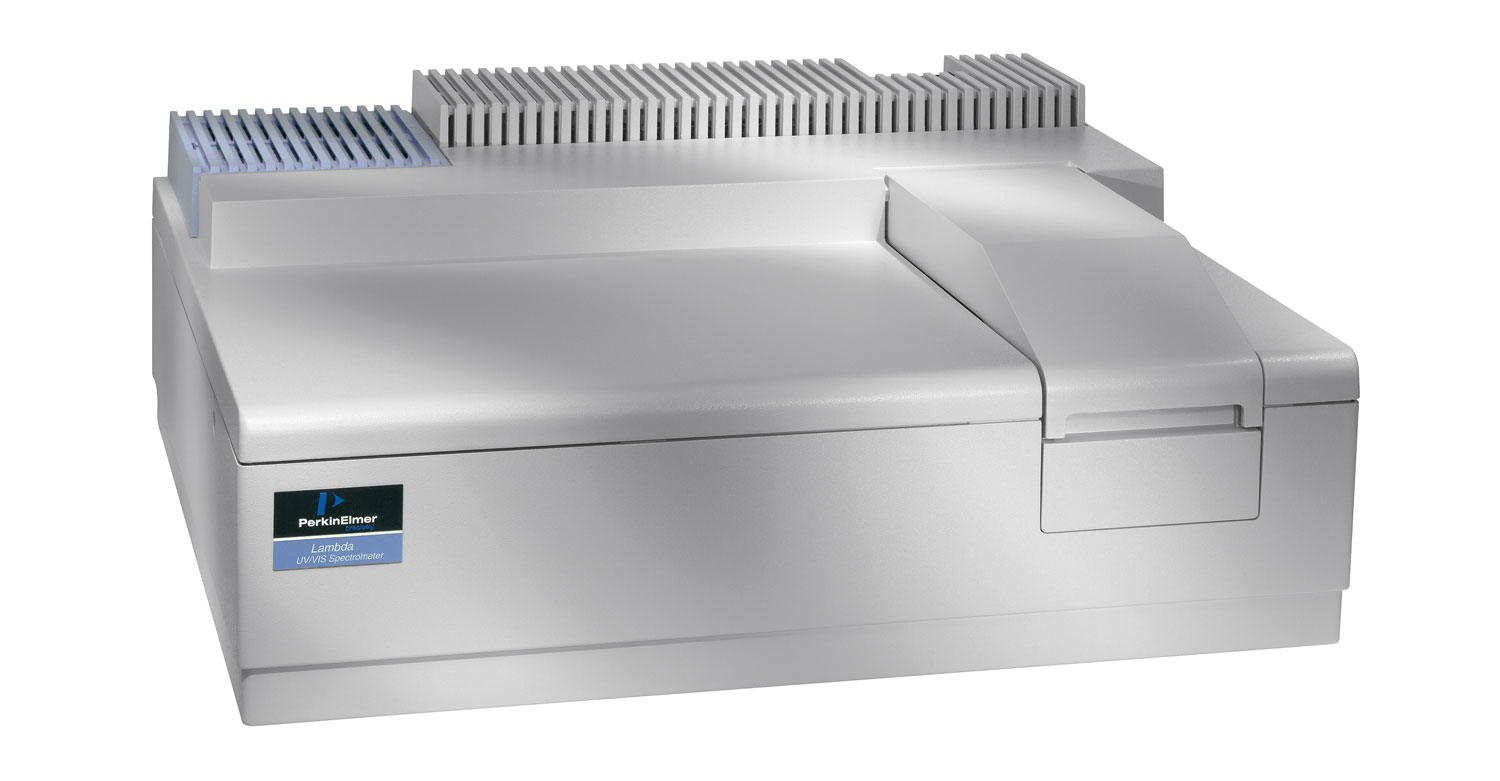
\includegraphics[width=120mm]{LAMBDA.jpg}
  \caption{Spektrofotometr LAMBDA 45 UV/Vis.}
  \label{lambdaimg}
\end{figure}




\subsection {Infračervená absorpční spektroskopie}
Záření v~IR oblasti nemá většinou dostatečnou energii k excitaci valenčních elektronů v~atomech, ale jeho energie je dostatečná pro změnu vibračního stavu molekuly vzorku. Samotné rotační a~vibrační stavy jsou kvantovou záležitostí a~pro jejich úplný popis potřebujeme kvantovou mechaniku. Pro zjednodušený popis a~schéma různých druhů vibrací se ale běžně používá klasická mechanika, kde o~molekule uvažujeme jako o~harmonickém oscilátoru.

Infračervené spektrum obsahuje absorpční píky, které odpovídají frekvenci vibrací molekul a~chemických skupin, jež tvoří materiál. Z IR spektroskopie tedy můžeme podle polohy píků identifikovat (kvalitativně) složení vzorku. Kromě toho velikost píků ve spektru obsahuje i informaci o~množství dané sloučeniny nebo skupiny.

Při měření IR spektra se většinou používá Fourierovská infračervená spektroskopie. Při FTIRu se místo mono\-chromátoru používá Michelsonův interferometr. V něm dochází k interferenci světla a měříme intenzity pro různé polohy zrcadla v interferometru. Výsledek, takzvaný interferogram, se na~počítači fourierovskou transformací převede na~spektrální závislost absorpce. Výhodou je výrazně větší rychlost měření.

\subsubsection{Bruker VERTEX 80v}
VERTEX 80v je vakuový FTIR spektrofotometr využívající Michelsonova interferometru, jehož zrcadlo kmitá na~vzduchovém polštáři. Byl použit speciální nástavec, jež umožňuje správné měření propustnosti. Vzorek byl při měření umístěn svisle na~držáku v~komoře, ze které byl vyčerpán vzduch na~2,51\,hPa. Vakuum je důležité kvůli eliminování vlivu prostředí a~atmosférické vlhkosti. Udávané spektrální rozlišení spektrometru je méně než než 0,2\,cm$^{-1}$. Infračervený spektrofotometr VERTEX 80v obsluhujeme pomocí programu OPUS. 

\begin{figure}
  \centering
  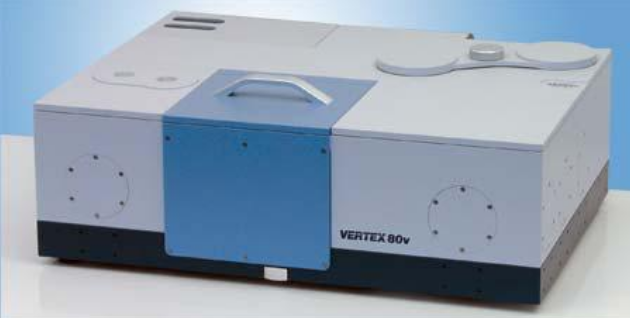
\includegraphics[width=120mm]{vertex80v.png}
  \caption{Spektrofotometr Bruker VERTEX 80v.}
  \label{verteximg}
\end{figure}


\section{Měření}

\subsection{Zpracování dat}
Pro zpracování dat byly použity některé programy vyvinuté na~fakultě, nainstalované na~počítači hercules. Pro odrazivost to byl program ,,spec''. Ten průměruje data z měření odrazivosti (v~našem případě 8 měření pro každý vzorek) a~přepočítává je proti uživatelem zvolenému normálu. Elipsometrická měření nebyla prováděna v~rámci praktika, ale byla použita již dříve naměřené data. Pro jejich zpracování byly použity programy ,,jy-rename.py'' a~,,ell'', které konvertují data z výstupního formátu elipsometru a ze sady měření na osmi konfiguracích počítají jednu trojici parametrů $I_\mathrm{s}$, $I_\mathrm{cII}$ a $I_\mathrm{cIII}$. 

Na~FTIRu byl každý vzorek měřen čtyřikrát a~po každém měření otočen o~90$^\circ$ stupňů (každé jednotlivé měření se skládalo ze 100 skenů). Na~začátku a~na~konci měření byl změřen tzv. background, tj. referenční signál bez přítomnosti vzorku. Relativní propustnost vrstvy se získá vydělením propustnosti vrstvy na~substrátu propustností samotného substrátu $T_\mathrm{rel} = T / T_\mathrm{Si}$. Propustnost vrstvy se substrátem byla získána jako aritmetický průměr z výše zmíněných čtyř měření, opravený o~referenční signál na~začátku a~na~konci měření. Výše uvedené operace byly provedeny programy ,,specIR-T'' a~,,awk''. Vrstva CH85a byla fitována programem newAD, pro ostatní vyhodnocování byly napsány vlastní programy. 


\subsection{Termální SiO$_2$ na~křemíku, který není k dispozici bez vrstvy (Si0$_2$Bl7)}
\subsubsection{Nafitování průměrné hodnoty odrazivosti v~UV/VIS pomocí vlastního programu za předpokladu normálového dopadu a~neabsorbující vrstvy (substrát je absorbující). Disperzní model indexu lomu uvažujme Cauchyho dvouparametrickou formuli. }

Při fitování vrstvy byl požit vzorec \ref{Rvzo}, disperzní model indexu lomu dle Cauchyho formule $n = A + \frac{B}{\lambda^2}$, bylo dosaženo výborné shody s experimentem (obrázek \ref{Sio2-R}). Index lomu vrstvy je na~obrázku \ref{Sio2n}. Určené parametry vrstvy jsou v~tabulce \ref{sio2fit}.

\begin{table}[htbp]
\begin{center}
\begin{tabular}{|c|c|c|}
\hline
$A$ & $B$ [nm$^2$] &  $d$ [nm] \\ \hline
1.4537 $\pm$ 0.0008 & 4003 $\pm$ 66 & 97.63 $\pm$ 0.08 \\ \hline
\end{tabular}
\caption{Fitované parametry vrstvy Si0$_2$Bl7. $A$,$B$ -- parametry Cauchyho formule, $d$ -- tloušťka vrstvy, interval spolehlivosti 68\,\%.}
\label{sio2fit}
\end{center}
\end{table}

\begin{figure}
  \centering
  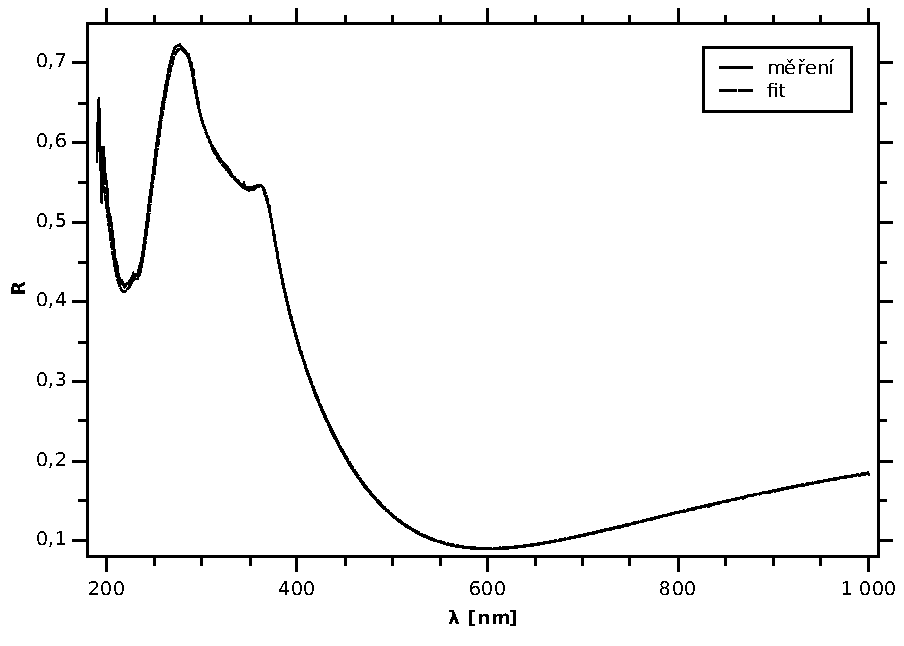
\includegraphics[width=135mm]{img/Sio2-R.pdf}
  \caption{Naměřená a~fitovaná odrazivost vrstvy Si0$_2$Bl7.}
  \label{Sio2-R}
\end{figure}

\begin{figure}
  \centering
  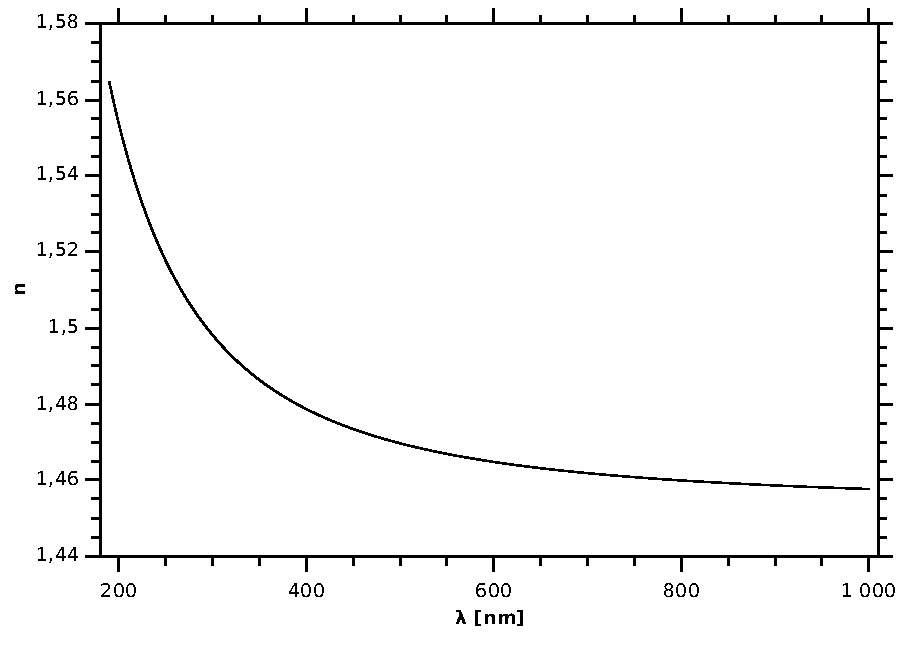
\includegraphics[width=135mm]{img/Sio2-n.pdf}
  \caption{Index lomu vrstvy Si0$_2$Bl7.}
  \label{Sio2n}
\end{figure}

\subsubsection{Posouzení propustnosti vzorku v~IR oblasti. V případě dostatečné propustnosti určení absorpčních píků. }
Při vyhodnocování propustnosti vzorku v~IR oblasti nebyl použit postup podělení propustnosti vzorku propustností substrátu, protože substrát byl v~tomto případě odlišný od ostatních vzorků (nebyl ze zadní strany vyleštěný) a~nebyl samostatně naměřen. Navíc, jak je vidět na~obrázku \ref{Sio2T}, je vzorek ve většině IR spektra nepropustný. Přesto můžeme v~oblasti nízkých vlnočtů identifikovat některé absorpční píky. Pík na~463\,cm$^{-1}$ přísluší kolébavým vibracím Si--O--Si. Pík na 1086\,cm$^{-1}$ je pravděpodobně složen ze dvou píků, jeden náleží valenčním vibracím Si--O--Si a druhý náleží substrátu (intersticiální kyslík). Pík na~610\,cm$^{-1}$ je multifononová absorpce v~křemíku. Píky křemíkového suibstrátu jsou podrobně popsány v tabulce \ref{SiIR}.

\begin{figure}
  \centering
  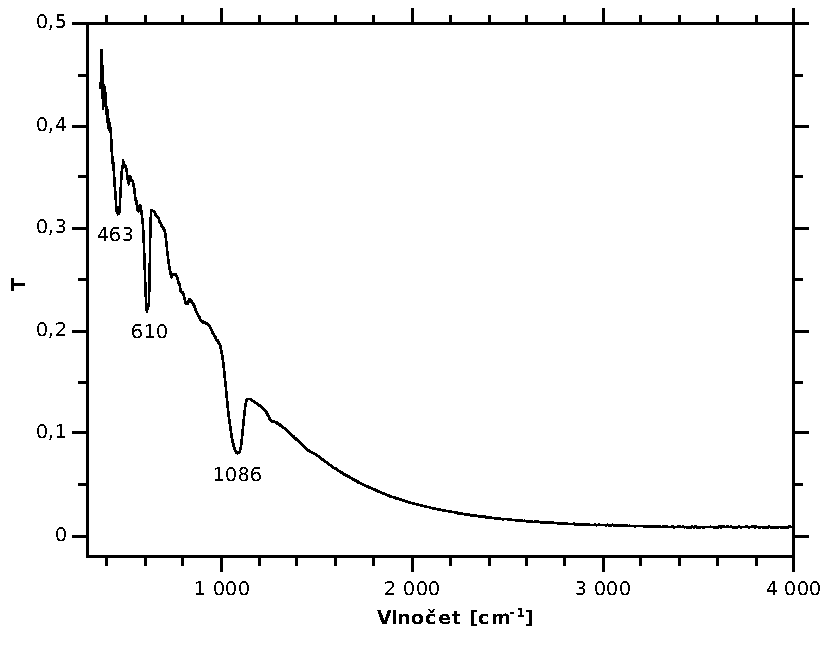
\includegraphics[width=130mm]{img/Sio2-T.pdf}
  \caption{Detail propustnosti vrstvy Si0$_2$Bl7.}
  \label{Sio2T}
\end{figure}





\subsection{Oboustranně leštěný křemík propustný v~IR oblasti (Si19-72) }
\subsubsection{Zprůměrování 4$\times$ měřené intenzity (single channel data) s opravou na~možnou změnu pozadí, tedy měření intenzity dopadajícího světla. Takto vypočítaná propustnost křemíku bude sloužit jako normalizační data pro výpočet relativní propustnosti vzorků s vrstvou. }

Na obrázku \ref{SiT} můžeme vidět získané absorpční spektrum křemíkového substrátu, které bylo dále používáno k výpočtům relativní propustnosti ostatních vzorků. Absorpční píky v~oblasti 400--1500\,cm$^{-1}$ (obrázek \ref{SiT2}) náleží fononovým absorpcím v~křemíku a~intersticiálnímu kyslíku, jejich identifikace je v tabulce \ref{SiIR}. Překvapivý je růst propustnosti v~oblasti 4000--7000\,cm$^{-1}$, toto je pravděpodobně způsobeno špatným nastavením měřícího přístroje.

\begin{table}[htbp]
\begin{center}
\begin{tabular}{|c|c|c|}
\hline
$\tilde{\nu}$ měřený [cm$^{-1}$] & $\tilde{\nu}$ tabulkový [cm$^{-1}$] & konfigurace \\ \hline
514 & 515 & multifononová absorpce (LO+TA)\\ \hline
514 & 515 & intersticiální kyslík \\ \hline
567 & 563 & multifononová absorpce (LO+TA) \\ \hline
612 & 610 & multifononová absorpce (TO+TA) \\ \hline
739 & 739 & multifononová absorpce (LO+LA) \\ \hline
820 & 817 & multifononová absorpce (TO+LA) \\ \hline
892 & 890 & multifononová absorpce (LO+TO) \\ \hline
1109 & 1107 & intersticiální kyslík \\ \hline
1297 & 1300 & intersticiální kyslík \\ \hline
1446 & 1450 & intersticiální kyslík) \\ \hline
\end{tabular}
\caption{Identifikované absorpční píky v~IR spektru křemíkového substrátu Si19-72. LO--podélný optický mód, TO--příčný optický mód, LA--podélný akustický mód, TA--příčný akustický mód.}
\label{SiIR}
\end{center}
\end{table}

\begin{figure}
  \centering
  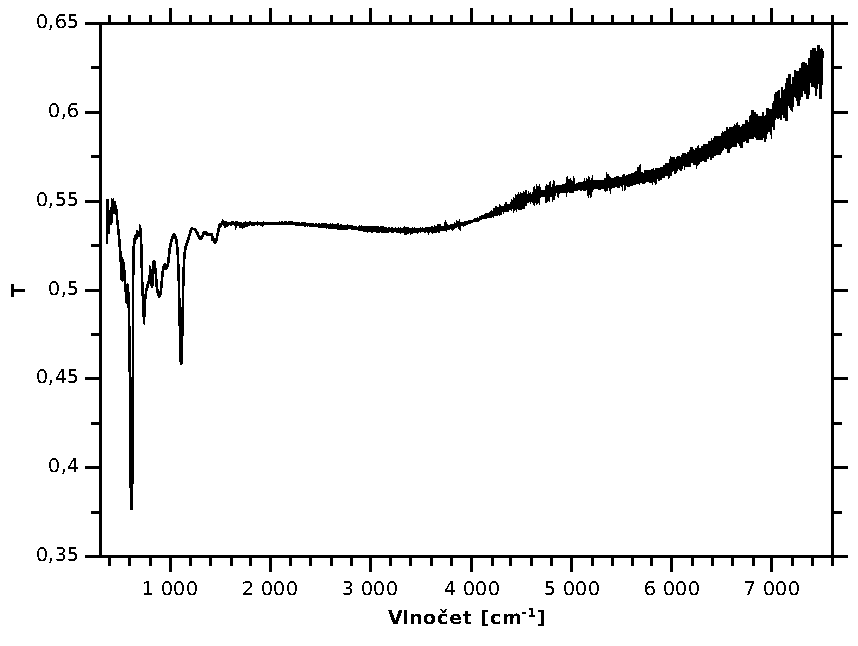
\includegraphics[width=135mm]{img/Si-T.pdf}
  \caption{Propustnost křemíkového substrátu Si19-72.}
  \label{SiT}
\end{figure}

\begin{figure}
  \centering
  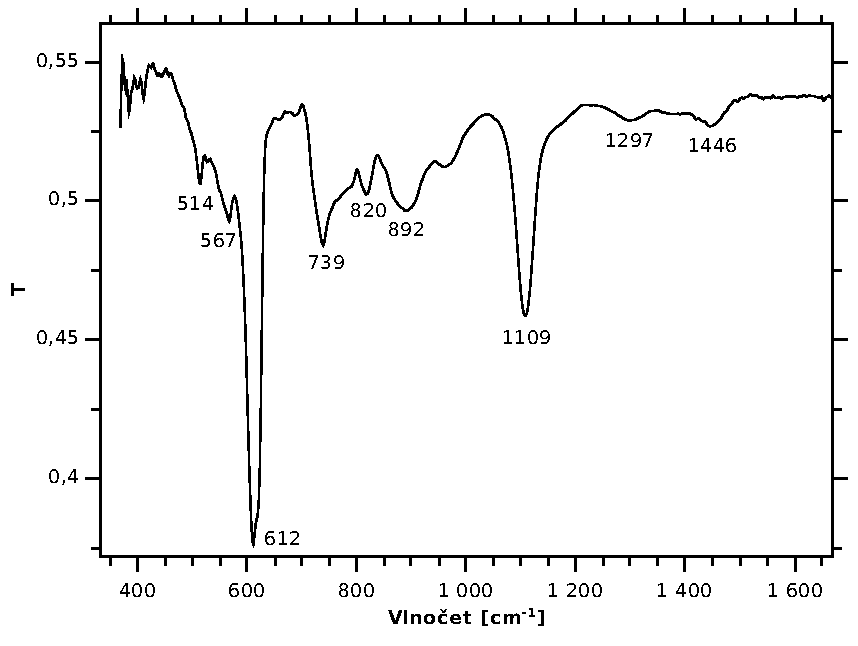
\includegraphics[width=135mm]{img/Si-T2.pdf}
  \caption{Detail propustnosti křemíkového substrátu Si19-72.}
  \label{SiT2}
\end{figure}







\subsection{Vrstva organosilikonového plazmového polymeru (SiOCH) připravená metodou PECVD na~křemíku (A50a) }
\subsubsection{Nafitování průměrné hodnoty odrazivosti v~UV/VIS oblasti pomocí vlastního programu jednak modelem neabsorbující vrstvy a~také za předpokladu slabé absorpce ve vrstvě. Disperzní model indexu lomu uvažujme Cauchyho dvouparametrickou formuli }

Měřená a~fitovaná odrazivost je na~obrázku \ref{A50a-R}. Je vidět, že model neabsorbující vrstvy se dobře shoduje s experimentálními daty s výjimkou UV oblasti, zde dává model se slabou absorpcí mnohem lepší výsledky. Extinkční koeficient byl předpokládán ve tvaru $k = \alpha \mathrm{e}^{-\beta \lambda}$. Fitované parametry vrstvy jsou v~tabulce \ref{Afit}. Získané optické konstanty pro oba modely jsou na~obrázku \ref{A50ank}.


\begin{table}[htbp]
\begin{center}
\begin{tabular}{|c|c|c|c|c|c|}
\hline
 & $A$ & $B$ [nm$^2$] &  $d$ [nm] & $\alpha$ & $\beta$ [10$^7$m$^{-1}$] \\ \hline
bez absorpce & 1.430 $\pm$ 0.001 & 5590 $\pm$ 120 & 114.27 $\pm$ 0.13 & - & - \\ \hline
slabá absorpce & 1.4277 $\pm$ 0.0005 & 6490 $\pm$ 60 & 114.09 $\pm$ 0.05 & 2030 $\pm$ 860 & 6.3 $\pm$ 0.2\\ \hline

\end{tabular}
\caption{Fitované parametry vrstvy A50a. $A$,$B$ -- parametry Cauchyho formule, $d$ -- tloušťka vrstvy, $\alpha$,$\beta$ -- parametry extinkčního koeficientu. Interval spolehlivosti 68\,\%.}
\label{Afit}
\end{center}
\end{table}

\begin{figure}
  \centering
  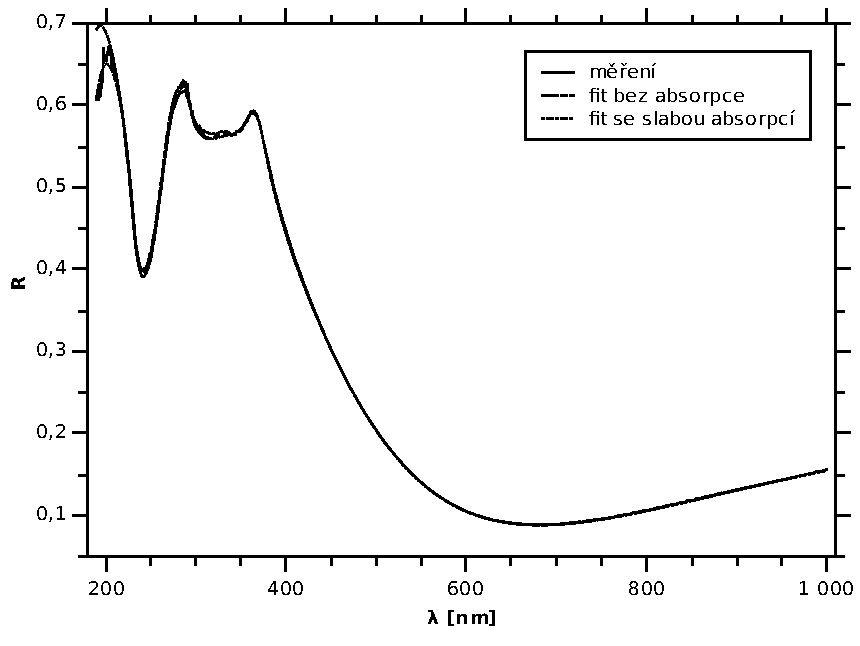
\includegraphics[width=135mm]{img/A50a-R.pdf}
  \caption{Naměřená a~fitovaná odrazivost vrstvy A50a.}
  \label{A50a-R}
\end{figure}

\begin{figure}
  \centering
  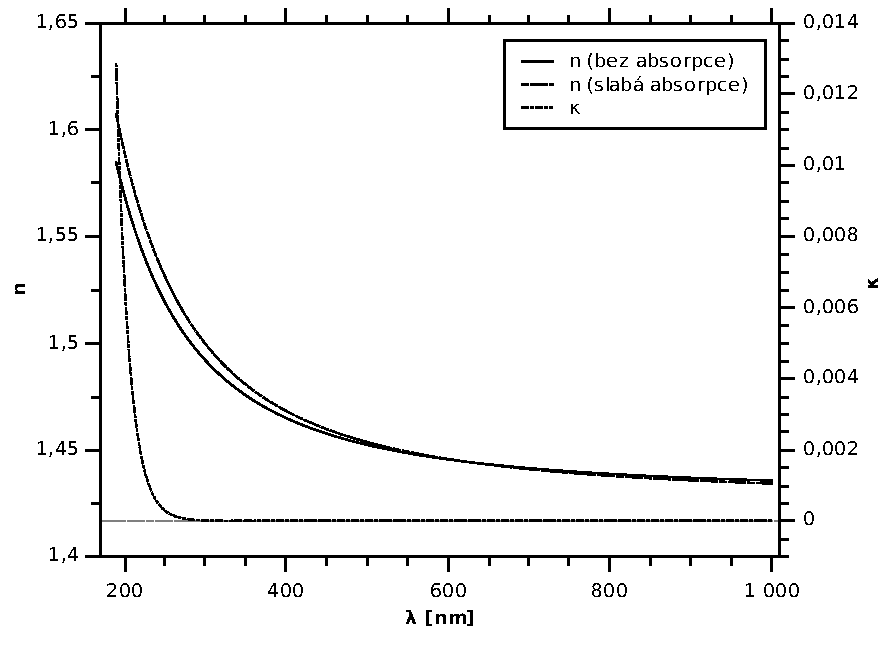
\includegraphics[width=135mm]{img/A50a-nk.pdf}
  \caption{Index lomu a~extinkční koeficient vrstvy A50a.}
  \label{A50ank}
\end{figure}

\subsubsection{Identifikace absorpčních píků v~UV oblasti }
Část infračerveného spektra vrstvy A50a je na~obrázku \ref{A50aIR}. Nejvýraznější pík na~1030\,cm$^{-1}$ patří valenčním vibracím skupiny Si--O--Si, další pík této skupiny (deformační) je na~798\,cm$^{-1}$. Také bychom očekávali ještě pík odpovídající kolébavým vibracím této skupiny na~450\,cm$^{-1}$, v~této oblasti je skutečně pík vidět, na cca 437\,cm$^{-1}$, ale určení jeho přesné polohy je obtížné kvůli tomu, že oblast pod 750\,cm$^{-1}$ bohužel obsahuje příliš mnoho šumu. Další výrazný pík je na~1261\,cm$^{-1}$, jsou to symetrické deformační vibrace skupiny Si-(CH$_3$)$_x$, pík příslušející asymetrickým deformačním vibracím stejné skupiny je na~1406\,cm$^{-1}$. Přitomnost těchto skupin je dále potvrzena píkem na~839\,cm$^{-1}$ (asymetrické valenční vibrace Si-(CH$_3$)$_x$), dále dříve zmíněný pík na~798\,cm$^{-1}$ může také náležet symetrickým valenčním vibracím této skupiny. Poslední dva výrazné píky (2905\,cm$^{-1}$ a~2962\,cm$^{-1}$) náleží symetrickým a~asymetrickým valenčním vibracím C-H v~CH$_3$. Všechny identifikované píky jsou shrnuty v~tabulce \ref{AIR}.

\begin{table}[htbp]
\begin{center}
\begin{tabular}{|c|c|c|}
\hline
$\tilde{\nu}$ měřený [cm$^{-1}$] & $\tilde{\nu}$ tabulkový [cm$^{-1}$] & skupina \\ \hline
437 & 450 & kolébavé vibrace Si--O--Si \\ \hline
798 & 800 & deformační vibrace Si--O--Si \\ \hline
798 & 800 & symetrické valenční vibrace Si-(CH$_3$)$_x$ \\ \hline
839 & 840 & asymetrické valenční vibrace Si-(CH$_3$)$_x$ \\ \hline
1030 & 1000-1100 & valenční asymetrické vibrace Si--O--Si \\ \hline
1261 & 1260 & symetrické deformační vibrace Si-(CH$_3$)$_x$ \\ \hline
1406 & 1410 & asymetrické deformační vibrace Si-(CH$_3$)$_x$ \\ \hline
2905 & 2910 & symetrické valenční vibrace C-H v~CH$_3$ \\ \hline
2962 & 2970 & asymetrické valenční vibrace C-H v~CH$_3$ \\ \hline
\end{tabular}
\caption{Identifikované absorpční píky v~IR spektru vrstvy A50a.}
\label{AIR}
\end{center}
\end{table}

\begin{figure}
  \centering
  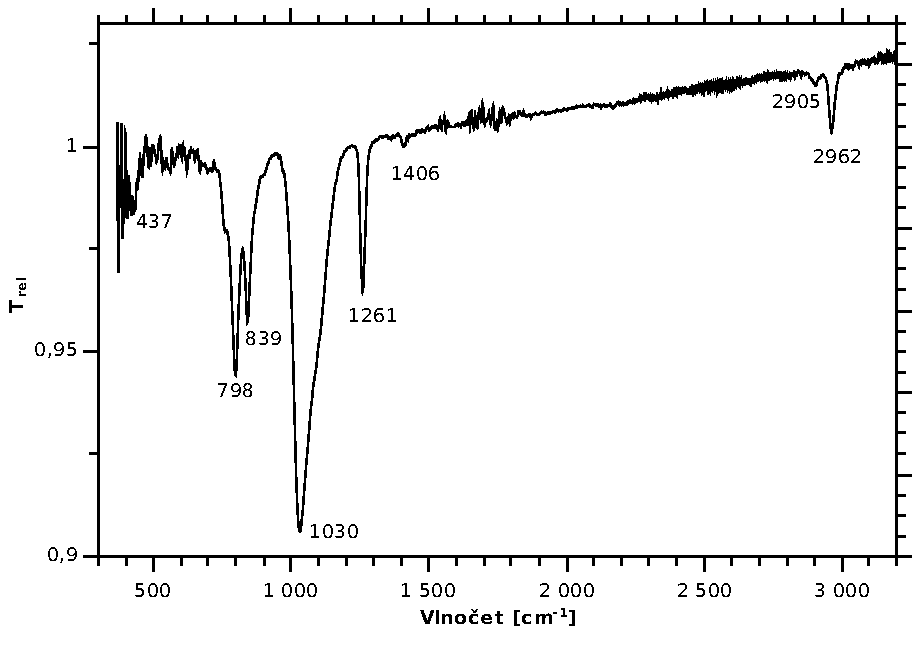
\includegraphics[width=135mm]{img/A50a-T.pdf}
  \caption{IR absorpční spektrum vrstvy A50a.}
  \label{A50aIR}
\end{figure}


\subsection{Vrstva diamantu podobného amorfního uhlíku (DLC) připravená metodou PECVD na~křemíku (CH85a)}
\subsubsection{Nafitování odrazivosti a~elipsometrických dat v~UV/VIS oblasti pomocí programu newAD a~vhodného disperzního modelu }

Vrstva CH85a byla fitována v~programu newAD modelem DLC. Získané optické konstanty jsou na~obrázku \ref{CH85nk}. Některé parametry DLC modelu jsou v~tabulce \ref{CHfit}. Opět se podařilo dosáhnout dobré shody fitu s měřením. Srovnání fitované a~měřené odrazivosti je na~obrázku \ref{CH85R}, fitované a~měřené přidružené elipsometrické parametry $I_\mathrm{s}$, $I_\mathrm{cII}$ a~$I_\mathrm{cIII}$ jsou na~obrázcích \ref{CH85is},\ref{CH85ic2} a~\ref{CH85ic3} (pro přehlednost jsou v~grafech pouze měření na~třech úhlech z celkových pěti).

\begin{table}[htbp]
\begin{center}
\begin{tabular}{|c|c|}
\hline
 $Q_\mathrm{\pi}$ [eV$^{-3/2}$] & 3.25 $\pm$ 0.08  \\ \hline
 $E_\mathrm{g\pi}$ [eV] & 1.401 $\pm$ 0.004 \\ \hline
 $E_\mathrm{h\pi}$ [eV] & 6.36 $\pm$ 0.01 \\ \hline 
 $Q_\mathrm{\sigma}$ [eV$^{-3/2}$] & 148 $\pm$ 2 \\ \hline
 $E_\mathrm{g\sigma}$ [eV] & 2.195 $\pm$ 0.005 \\ \hline
 $E_\mathrm{h\sigma}$ [eV] & 51.9 $\pm$ 0.6 \\ \hline
 $d_\mathrm{e}$ [nm] & 416.1 $\pm$ 0.2 \\ \hline
 $d_\mathrm{r}$ [nm] & 413.1 $\pm$ 0.36 \\ \hline
\end{tabular}
\caption{Fitované parametry vrstvy CH85a. $d_\mathrm{e}$, $d_\mathrm{r}$ -- tloušťky vrstvy na~elipsometrii a~odrazivosti. $Q_\mathrm{\pi}$,$Q_\mathrm{\sigma}$ -- parametry úměrné koncentraci $\pi$ a~$\sigma$ elektronů. $E_\mathrm{g\pi}$,$E_\mathrm{g\sigma}$ šířka zakázaného pásu $\pi$ a~$\sigma$ elektronů. $E_\mathrm{h\pi}$,$E_\mathrm{h\sigma}$ maximální energie mezipásových přechodů $\pi$ a~$\sigma$ elektronů.   }
\label{CHfit}
\end{center}
\end{table}

\begin{figure}
  \centering
  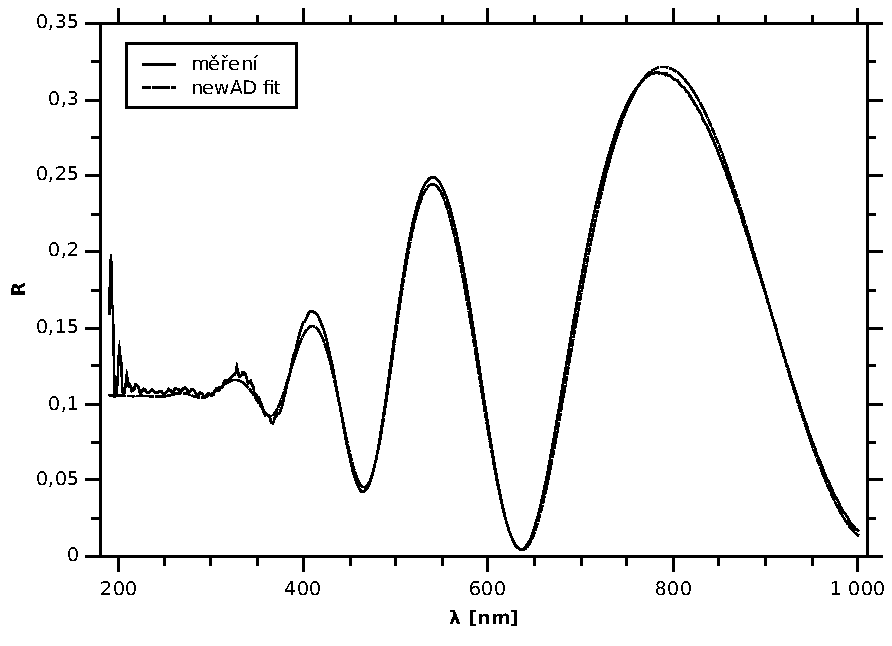
\includegraphics[width=135mm]{img/CH85-R.pdf}
  \caption{Naměřená a~fitovaná odrazivost vrstvy CH85a.}
  \label{CH85R}
\end{figure}

\begin{figure}
  \centering
  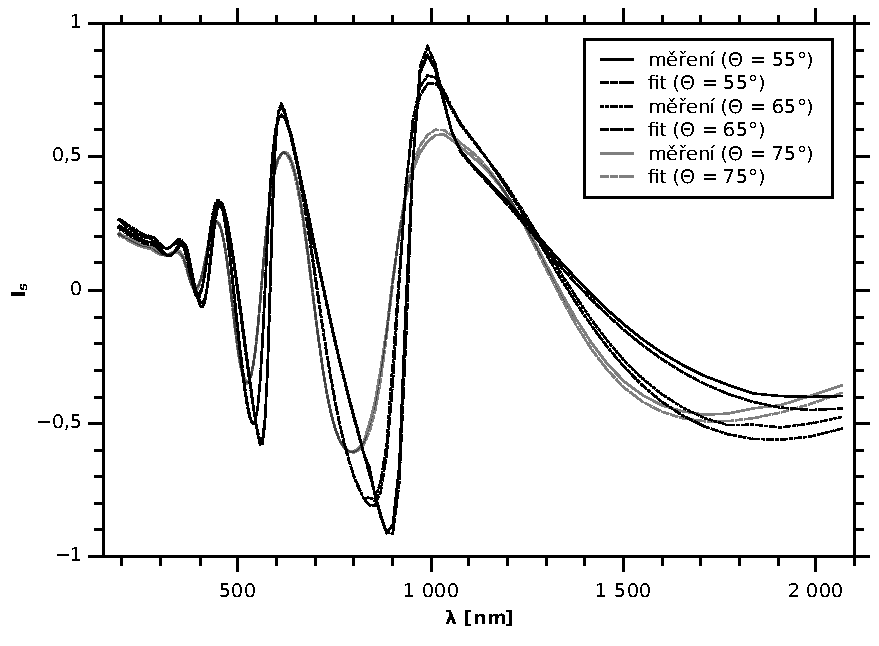
\includegraphics[width=135mm]{img/CH85-is1.pdf}
  \caption{Přidružený elipsometrický parametr $I_\mathrm{s}$ vrstvy CH85a (pro 3 úhly měření).}
  \label{CH85is}
\end{figure}

\begin{figure}
  \centering
  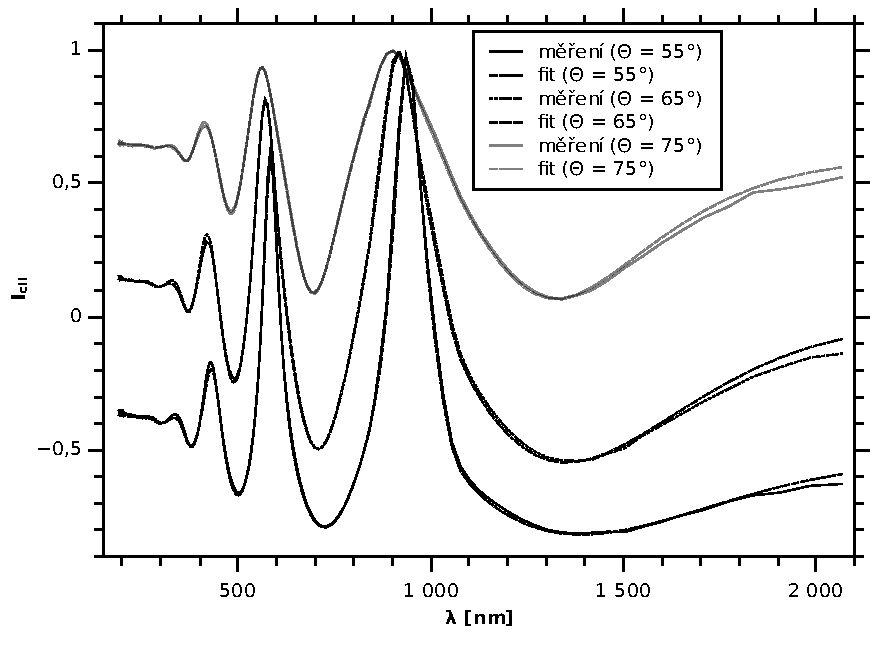
\includegraphics[width=135mm]{img/CH85-ic2.pdf}
  \caption{Přidružený elipsometrický parametr $I_\mathrm{cII}$ vrstvy CH85a (pro 3 úhly měření).}
  \label{CH85ic2}
\end{figure}

\begin{figure}
  \centering
  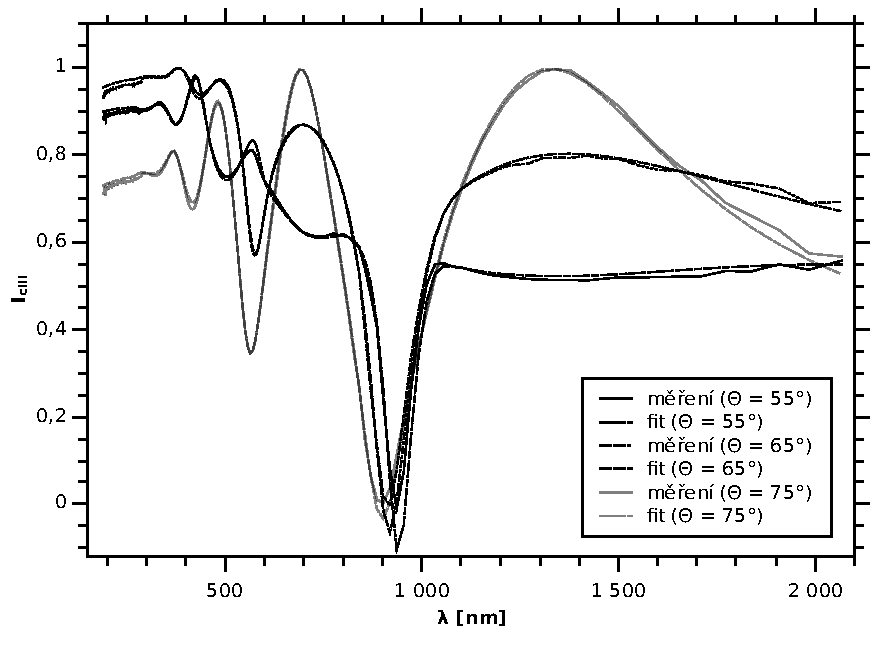
\includegraphics[width=135mm]{img/CH85-ic3.pdf}
  \caption{Přidružený elipsometrický parametr $I_\mathrm{cIII}$ vrstvy CH85a (pro 3 úhly měření).}
  \label{CH85ic3}
\end{figure}

\begin{figure}
  \centering
  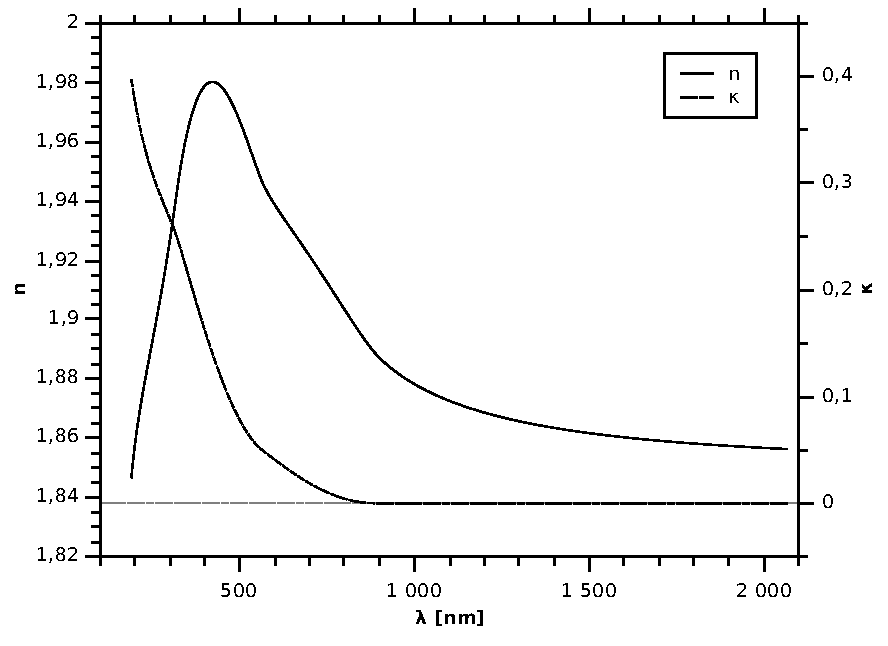
\includegraphics[width=135mm]{img/CH85-nk.pdf}
  \caption{Index lomu a~extinkční koeficient vrstvy CH85a získané programem newAD.}
  \label{CH85nk}
\end{figure}

\subsubsection{Určení dielektrické funkce vrstvy přímo z elipsometrických měření za předpokladu polonekonečné vrstvy (silná absorpce ve vrstvě)}

Index lomu (obrázek \ref{CH85n}) a~extinkční koeficient (obrázek \ref{CH85k}) byly určeny dle vzorce \ref{ellrov}, dielektrická funkce (obrázky \ref{CH85Ree}, \ref{CH85Ime}) byla následně dopočítána podle vzorce $\hat{\epsilon} = \hat{n}^2$. Z grafů je vidět, že model polonekonečné vrstvy nedává v~tomto případě dobré výsledky, to je způsobené tím, že nelze zanedbat zpětný odraz na~rozhraní substrát--vrstva (vrstva není dostatečně tlustá a~absorbující).

\begin{figure}
  \centering
  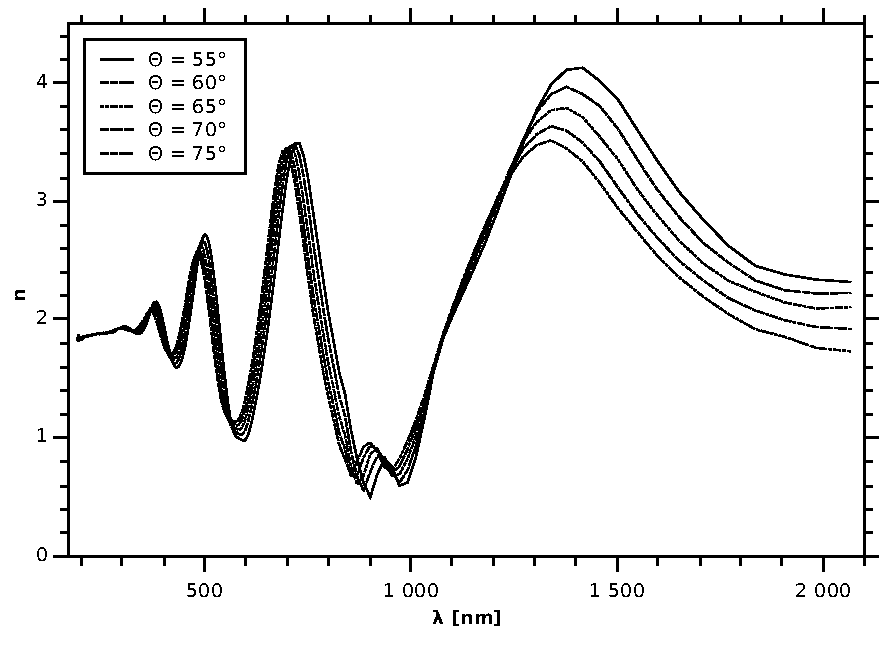
\includegraphics[width=135mm]{img/CH85-n.pdf}
  \caption{Index lomu vrstvy CH85a za předpokladu polonekonečné vrstvy.}
  \label{CH85n}
\end{figure}

\begin{figure}
  \centering
  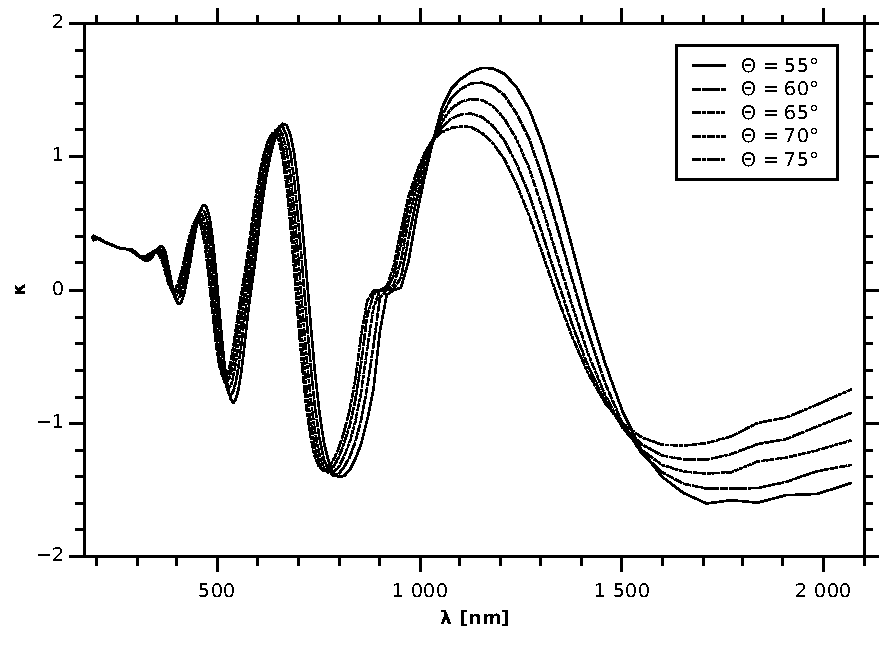
\includegraphics[width=135mm]{img/CH85-k.pdf}
  \caption{Extinkční koeficient vrstvy CH85a za předpokladu polonekonečné vrstvy.}
  \label{CH85k}
\end{figure}

\begin{figure}
  \centering
  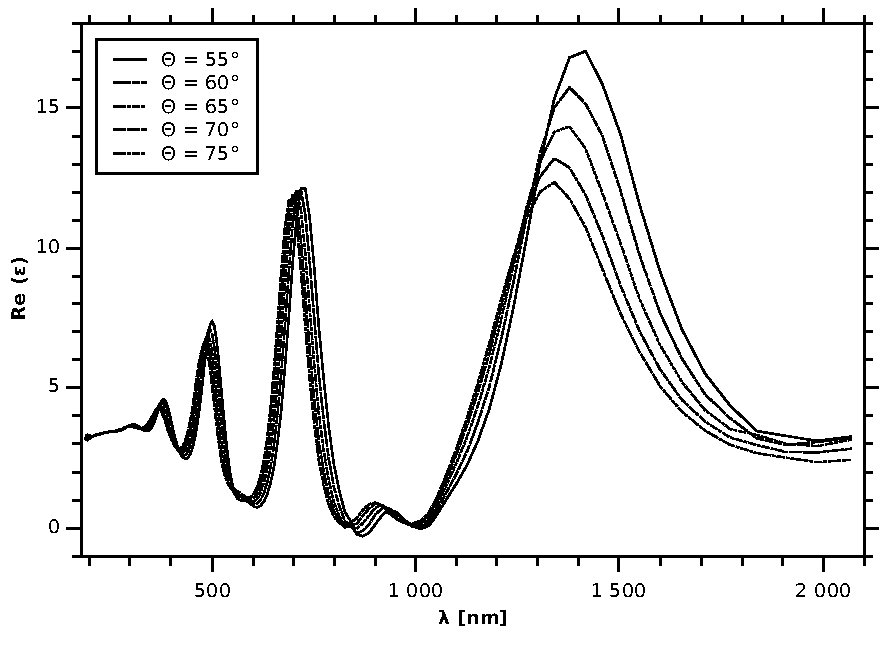
\includegraphics[width=135mm]{img/CH85-Ree.pdf}
  \caption{Reálná část dielektrické funkce vrstvy CH85a za předpokladu polonekonečné vrstvy.}
  \label{CH85Ree}
\end{figure}

\begin{figure}
  \centering
  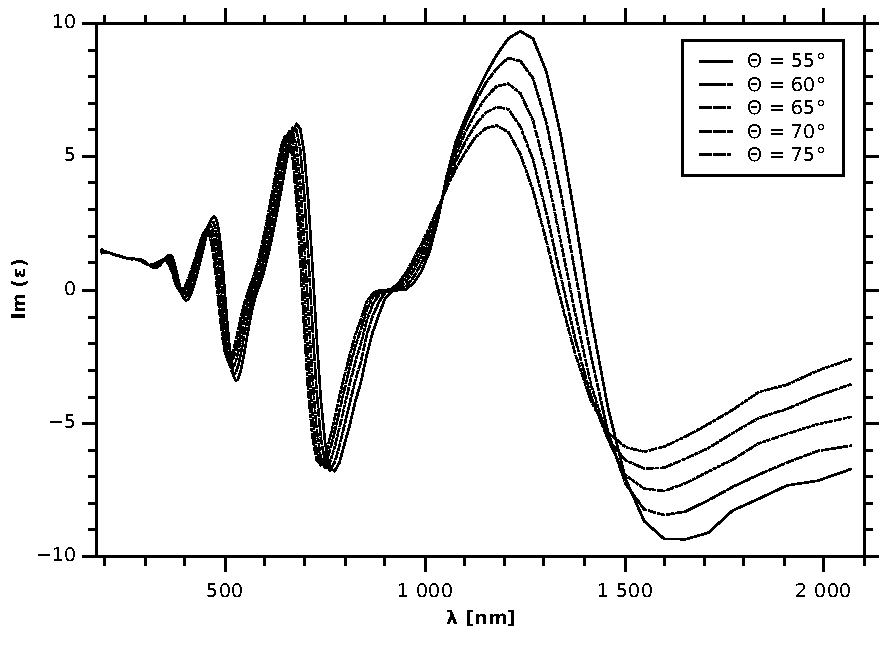
\includegraphics[width=135mm]{img/CH85-Ime.pdf}
  \caption{Imaginární část dielektrické funkce vrstvy CH85a za předpokladu polonekonečné vrstvy.}
  \label{CH85Ime}
\end{figure}


\subsubsection{Identifikace absorpčních píků v~IR oblasti }
Naměřené IR spektrum je na~obrázku \ref{CH85aIR}. Analýza tohoto spektra není jednoznačná. Jednak je v~něm hodně šumu, navíc jsou ve spektru pouze dva výrazné píky. Jeden v~oblasti 2800--3050\,cm$^{-1}$, který je ve skutečnosti složen z cca 9 různých píků (příslušejících valenčním sp$^{2,3}$C--H$_{1,2,3}$ vibracím). Tyto jsou uvedeny v~tabulce \ref{CH85IR}, ovšem intenzita jednotlivých píků, případně jestli jsou vůbec zastoupeny se nedá bez fitování IR spektra odhadnout. Druhý výrazní pík je na~1444\,cm$^{-1}$, to může být některá deformační vibrace skupiny sp$^3$C--H$_x$, možné vibrační módy jsou opět uvedeny v~tabulce \ref{CH85IR}. Téměř neznatelný pík na~1374\,cm$^{-1}$ jsou symetrické deformační vibrace sp$^3$C--H$_3$. Další malý široký pík je v~oblasti 1540--1650\,cm$^{-1}$, jedná se pravděpodobně o~vibrace skupiny sp$^2$C. Oblast pod 1000\,cm$^{-1}$ nemá smysl podrobně zkoumat, protože v~této oblasti silně absorbuje křemík a~použitá metoda vydělení propustnosti vzorku propustností substrátu zde není schopna dobře odstranit vliv substrátu.
 
\begin{table}[htbp]
\begin{center}
\begin{tabular}{|c|c|c|}
\hline
$\tilde{\nu}$ měřený [cm$^{-1}$] & $\tilde{\nu}$ tabulkový [cm$^{-1}$] & vibrační mód \\ \hline
1374 & 1375 & sp$^3$C--H$_3$ sym. bend. \\ \hline
1444 & 1450 & sp$^3$C--H$_2$ scissoring \\ \hline
1444 & 1460 & sp$^3$C--H$_3$ asym. bend. \\ \hline
1540-1650 & 1600 & sp$^2$C \\ \hline
2800--3050 & 2855 & sp$^3$C--H$_2$ sym.  \\ \hline  
2800--3050 & 2870 & sp$^3$C--H$_3$ sym.  \\ \hline  
2800--3050 & 2915 & sp$^3$C--H  \\ \hline
2800--3050 & 2925 & sp$^3$C--H$_2$ asym.  \\ \hline
2800--3050 & 2960 & sp$^3$C--H$_3$ asym.  \\ \hline
2800--3050 & 3000 & sp$^2$C--H$_2$ olef. asym.  \\ \hline
2800--3050 & 3030 & sp$^2$C--H olef.  \\ \hline
2800--3050 & 3050 & sp$^2$C--H arom.  \\ \hline
2800--3050 & 3080 & sp$^2$C--H$_2$ olef. sym.  \\ \hline
\end{tabular}
\caption{Možné absorpční píky v~IR spektru vrstvy CH85a.}
\label{CH85IR}
\end{center}
\end{table}

\begin{figure}
  \centering
  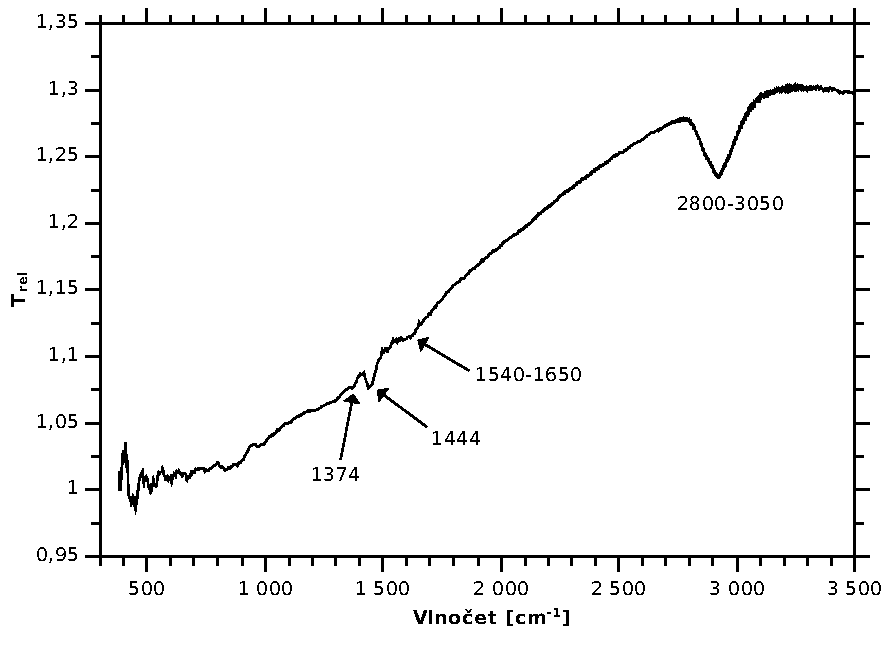
\includegraphics[width=135mm]{img/CH85-T.pdf}
  \caption{IR absorpční spektrum vrstvy CH85a.}
  \label{CH85aIR}
\end{figure}



\newpage

\subsection{Vrstva železa připravená na~zlaté vrstvě na~Si, oboje metodou PLD}
\subsubsection{Určení dielektrické funkce vrstvy přímo z elipsometrických měření za předpokladu polonekonečné vrstvy (silná absorpce ve vrstvě)}

Index lomu (obrázek \ref{Aun}) a~extinkční koeficient (obrázek \ref{Auk}) byly určeny dle vzorce \ref{ellrov}, dielektrická funkce (obrázky \ref{AuRee}, \ref{AuIme}) byla následně dopočítána podle vzorce $\hat{\epsilon} = \hat{n}^2$. Je vidět, že v~tomto případě jsme se předpokladem polonekonečné vrstvy nedopustili velké chyby, výsledky jsou velmi podobné pro různé úhly dopadu a~index lomu i extinkční koeficient jsou nezáporné, na~rozdíl od vrstvy CH85a.

\begin{figure}
  \centering
  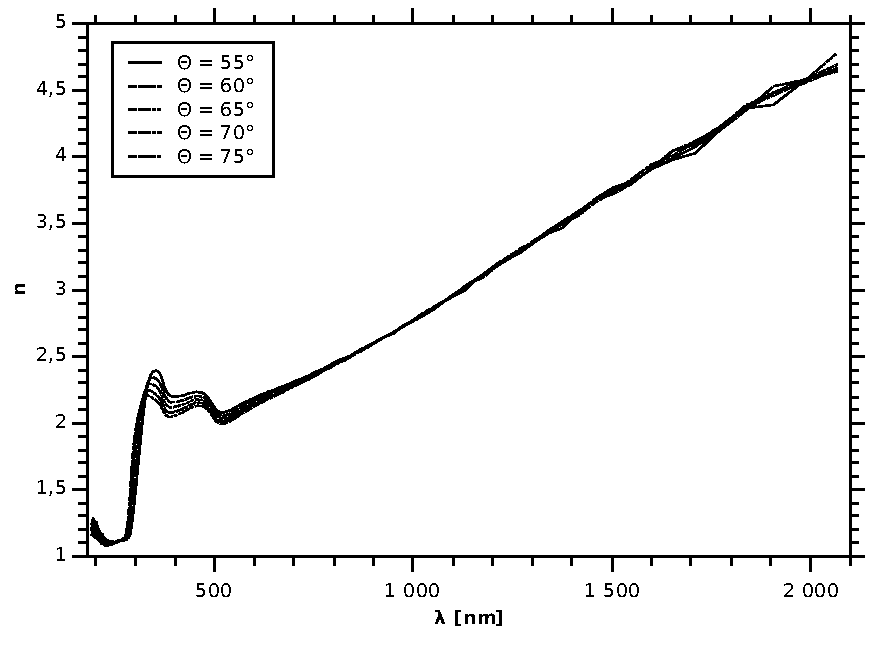
\includegraphics[width=135mm]{img/Au-n.pdf}
  \caption{Index lomu vrstvy Au57Fe-2.}
  \label{Aun}
\end{figure}

\begin{figure}
  \centering
  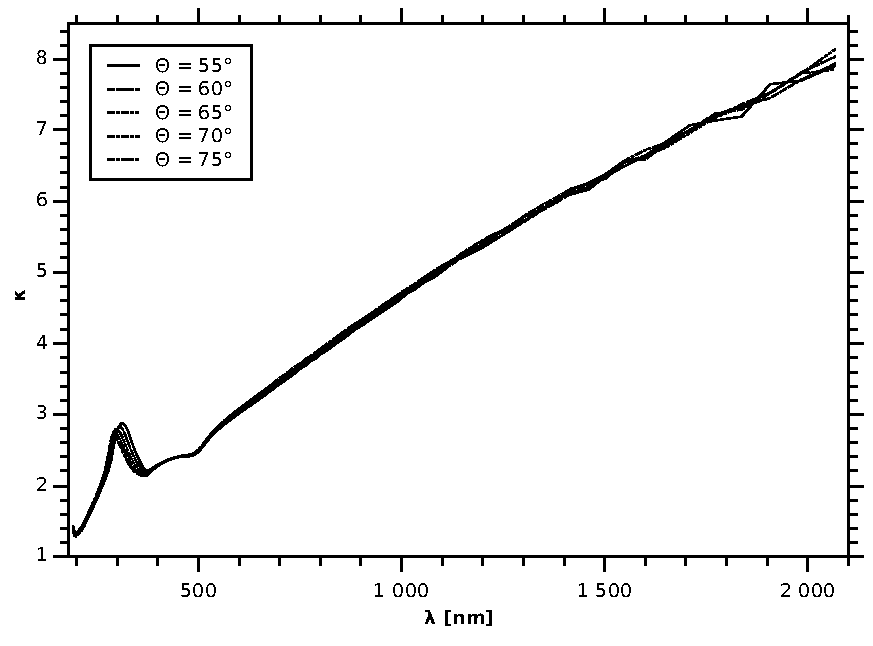
\includegraphics[width=135mm]{img/Au-k.pdf}
  \caption{Extinkční koeficinet vrstvy Au57Fe-2.}
  \label{Auk}
\end{figure}

\begin{figure}
  \centering
  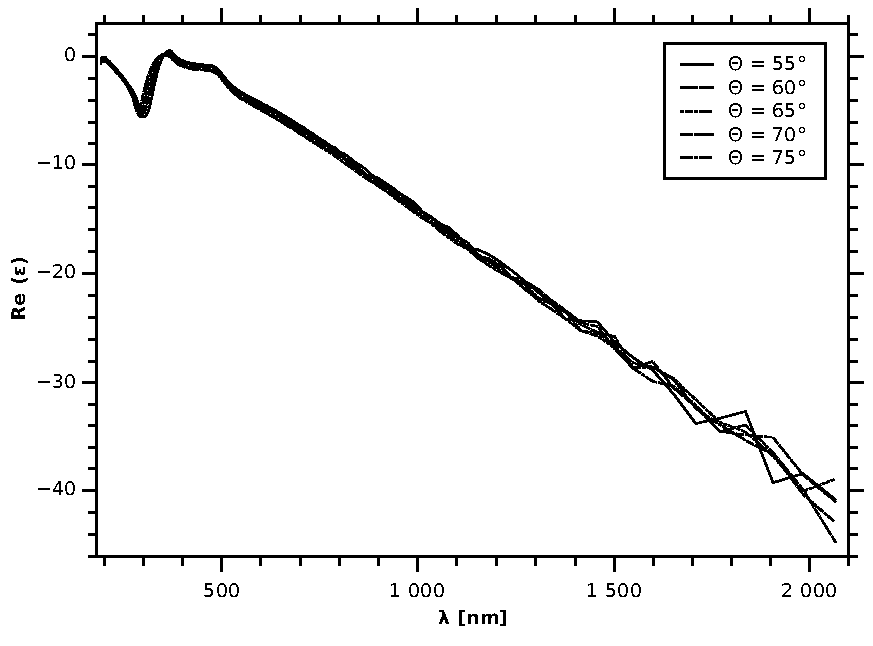
\includegraphics[width=135mm]{img/Au-Ree.pdf}
  \caption{Reálná část dielektrické funkce vrstvy Au57Fe-2.}
  \label{AuRee}
\end{figure}

\begin{figure}
  \centering
  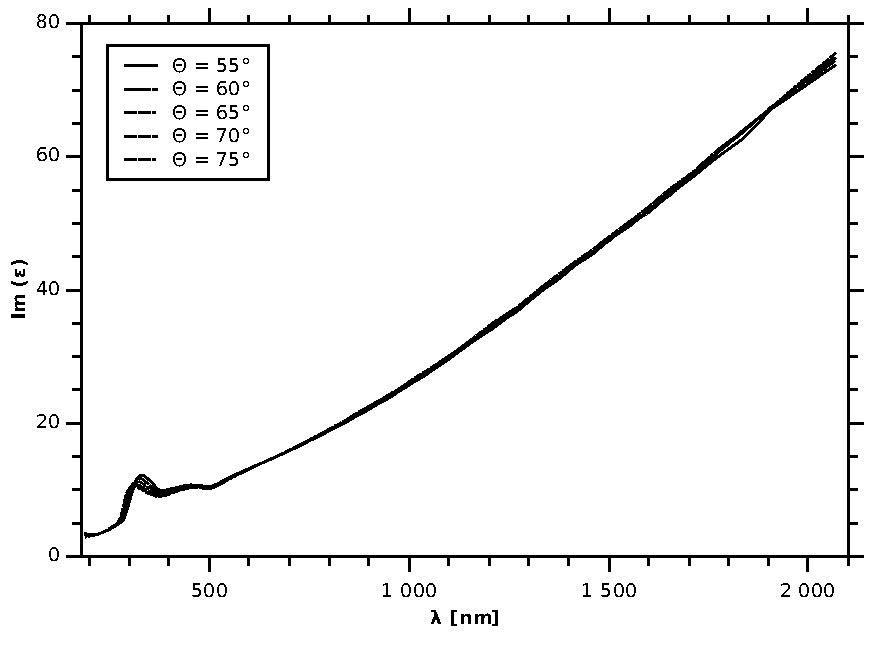
\includegraphics[width=135mm]{img/Au-Ime.pdf}
  \caption{Imaginární část dielektrické funkce vrstvy Au57Fe-2.}
  \label{AuIme}
\end{figure}

\section{Závěr}
Praktikum proběhlo úspěšně. Podařilo se naměřit a~vyhodnotit všechny požadované veličiny. Také zpracování dat proběhlo v~pořádku. Ukázalo se, že ve většině případů vystačíme při analýze vrstev s jednoduchými modely odrazivosti (termální SiO$_2$, organosilikonová polymerní vrstva A50a), případně elipsometrie (vrstva železa na~zlatě na~křemíku). Pouze pro vrstvu DLC bylo potřeba při fitování použít složitější model (z programu newAD), protože jednoduché nedávaly uspokojivé výsledky. DLC vrstva se ukázala jako komplikovaná i při vyhodnocování absorpce v~IR oblasti, kvůli šumu a~malé velikosti absorpčních píků. Analýza IR absorpčního spektra vrstvy A50a proběhla naopak bez problémů. Ve všech IR spektrech se navíc ukázalo neobvyklé zvýšení propustnosti pro vysoké vlnočty, toto bylo pravděpodobně způsobeno špatným nastavením spektrofotometru. Naštěstí v~oblasti, kde k tomuto docházelo, nebyly žádné absorpční píky přítomny. 

\end{document}
